% !TEX root = ./proj_report.tex
\graphicspath{{put_your_path/}}% Set graphics path location

\chapter{Filter Characteristics}
 Choice of filter is very important in image restoration and restored image characteristics. This part of the project aims to study different filters and compare their enhancement effectiveness and deblur characteristics under various simulated and real image blur phenomenon. Before we present a comparison, let us briefly discuss the different filters studied for the purposes of this project. Various filters compared are, 
\begin{enumerate}
\item Inverse and Pseudo filter
\item Wiener filter
\item Geometric mean filter
\item Constrained least squares filter
\end{enumerate} 
Mathematical formulation of these filters has been presented in the Appendix and will not be discussed here. 
\section{Train Image: Supersonic flow around a sphere}
In this simulated motion blur, train image was procured from Van Dyke's Album of Fluid Motion and depicts the formation of shock around a sphere at flow Mach no. 3. This image was blurred using a motion PSF and had Gaussian white additive noise. The blurred image and recovered image are presented below. Filter deblur characteristics follow below.

\begin{figure}
        \centering
        \begin{subfigure}[b]{0.4\textwidth}
                \centering
                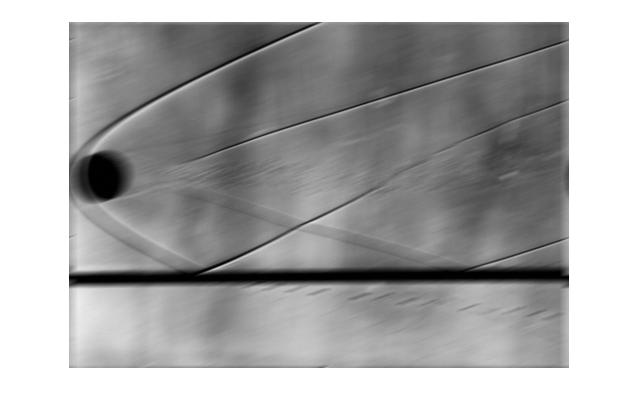
\includegraphics[width=\textwidth]{/Users/mehuloswal/me354_final_project/report/part1_figs/ssphere_motion.jpg}
                \caption{Blurry image}
                
        \end{subfigure}
        \begin{subfigure}[b]{0.4\textwidth}
                \centering
                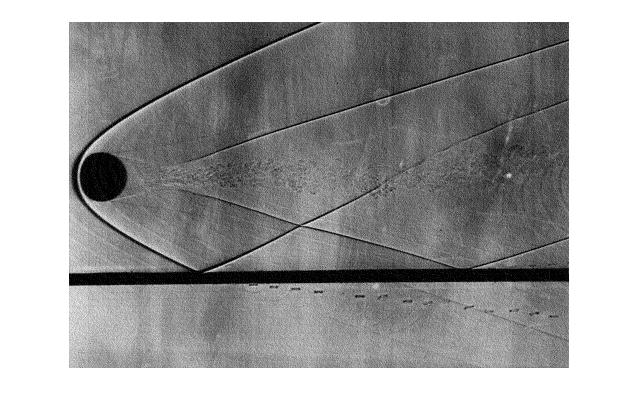
\includegraphics[width=\textwidth]{/Users/mehuloswal/me354_final_project/report/part1_figs/ssphere_wiener.jpg}
                \caption{Wiener filter sharpened image} 
        \end{subfigure}
\caption{Image enhancement on the blurred image was performed using all the filters. For representative purposes only the sharpened image using Wiener filter has been shown here. Blur PSF used for this simulation represented blur effect due to motion. Variance of the additive noise is of $O(10^{-5}$. }
\end{figure}

\begin{figure}[h!]
  \centering
                \centering
                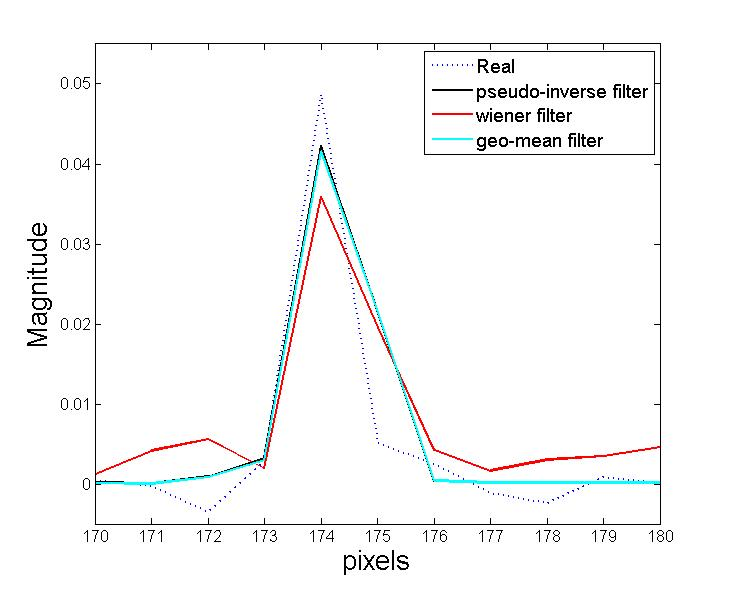
\includegraphics[width=.5\textwidth]{/Users/mehuloswal/me354_final_project/report/part1_figs/kernel_motion.jpg}
                \caption{Kernel comparison for blur due to motion}
                \end{figure}

\begin{figure}
        \centering
        \begin{subfigure}[b]{0.4\textwidth}
                \centering
                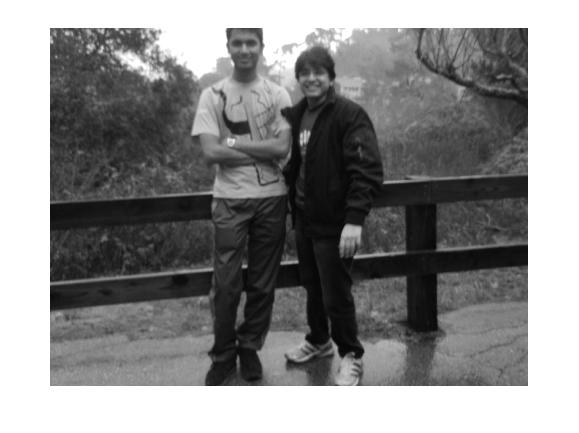
\includegraphics[width=\textwidth]{/Users/mehuloswal/me354_final_project/report/part1_figs/blur_personal.jpg}
                \caption{No reference blurry image}
                
        \end{subfigure}
        \begin{subfigure}[b]{0.4\textwidth}
                \centering
                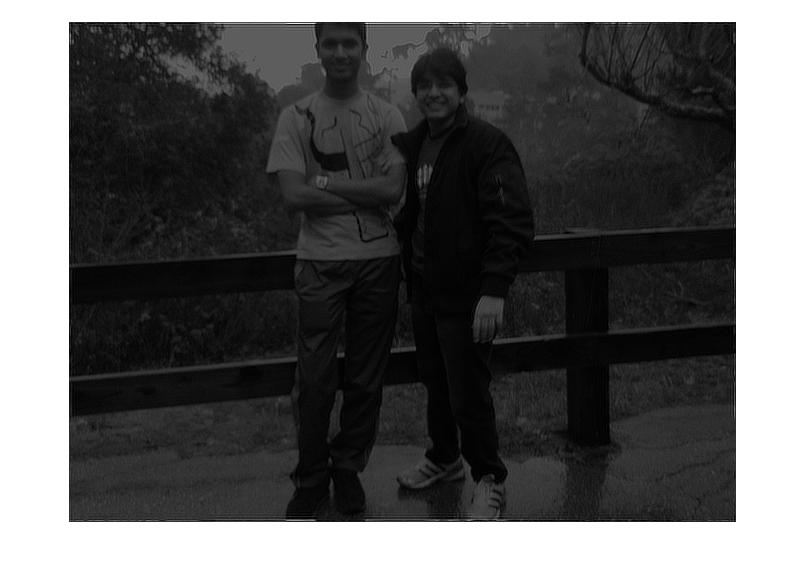
\includegraphics[width=\textwidth]{/Users/mehuloswal/me354_final_project/report/part1_figs/sharp_personal.jpg}
                \caption{Wiener filter sharpened image} 
        \end{subfigure}
\caption{No reference image enhancement}
\end{figure}

\newpage